\documentclass[]{book}
\usepackage{lmodern}
\usepackage{amssymb,amsmath}
\usepackage{ifxetex,ifluatex}
\usepackage{fixltx2e} % provides \textsubscript
\ifnum 0\ifxetex 1\fi\ifluatex 1\fi=0 % if pdftex
  \usepackage[T1]{fontenc}
  \usepackage[utf8]{inputenc}
\else % if luatex or xelatex
  \ifxetex
    \usepackage{mathspec}
  \else
    \usepackage{fontspec}
  \fi
  \defaultfontfeatures{Ligatures=TeX,Scale=MatchLowercase}
\fi
% use upquote if available, for straight quotes in verbatim environments
\IfFileExists{upquote.sty}{\usepackage{upquote}}{}
% use microtype if available
\IfFileExists{microtype.sty}{%
\usepackage{microtype}
\UseMicrotypeSet[protrusion]{basicmath} % disable protrusion for tt fonts
}{}
\usepackage[margin=1in]{geometry}
\usepackage{hyperref}
\hypersetup{unicode=true,
            pdftitle={Applied Error Modeling in Regression},
            pdfauthor={Stefanie Muff and Lukas F. Keller},
            pdfborder={0 0 0},
            breaklinks=true}
\urlstyle{same}  % don't use monospace font for urls
\usepackage{natbib}
\bibliographystyle{apalike}
\usepackage{color}
\usepackage{fancyvrb}
\newcommand{\VerbBar}{|}
\newcommand{\VERB}{\Verb[commandchars=\\\{\}]}
\DefineVerbatimEnvironment{Highlighting}{Verbatim}{commandchars=\\\{\}}
% Add ',fontsize=\small' for more characters per line
\usepackage{framed}
\definecolor{shadecolor}{RGB}{248,248,248}
\newenvironment{Shaded}{\begin{snugshade}}{\end{snugshade}}
\newcommand{\KeywordTok}[1]{\textcolor[rgb]{0.13,0.29,0.53}{\textbf{#1}}}
\newcommand{\DataTypeTok}[1]{\textcolor[rgb]{0.13,0.29,0.53}{#1}}
\newcommand{\DecValTok}[1]{\textcolor[rgb]{0.00,0.00,0.81}{#1}}
\newcommand{\BaseNTok}[1]{\textcolor[rgb]{0.00,0.00,0.81}{#1}}
\newcommand{\FloatTok}[1]{\textcolor[rgb]{0.00,0.00,0.81}{#1}}
\newcommand{\ConstantTok}[1]{\textcolor[rgb]{0.00,0.00,0.00}{#1}}
\newcommand{\CharTok}[1]{\textcolor[rgb]{0.31,0.60,0.02}{#1}}
\newcommand{\SpecialCharTok}[1]{\textcolor[rgb]{0.00,0.00,0.00}{#1}}
\newcommand{\StringTok}[1]{\textcolor[rgb]{0.31,0.60,0.02}{#1}}
\newcommand{\VerbatimStringTok}[1]{\textcolor[rgb]{0.31,0.60,0.02}{#1}}
\newcommand{\SpecialStringTok}[1]{\textcolor[rgb]{0.31,0.60,0.02}{#1}}
\newcommand{\ImportTok}[1]{#1}
\newcommand{\CommentTok}[1]{\textcolor[rgb]{0.56,0.35,0.01}{\textit{#1}}}
\newcommand{\DocumentationTok}[1]{\textcolor[rgb]{0.56,0.35,0.01}{\textbf{\textit{#1}}}}
\newcommand{\AnnotationTok}[1]{\textcolor[rgb]{0.56,0.35,0.01}{\textbf{\textit{#1}}}}
\newcommand{\CommentVarTok}[1]{\textcolor[rgb]{0.56,0.35,0.01}{\textbf{\textit{#1}}}}
\newcommand{\OtherTok}[1]{\textcolor[rgb]{0.56,0.35,0.01}{#1}}
\newcommand{\FunctionTok}[1]{\textcolor[rgb]{0.00,0.00,0.00}{#1}}
\newcommand{\VariableTok}[1]{\textcolor[rgb]{0.00,0.00,0.00}{#1}}
\newcommand{\ControlFlowTok}[1]{\textcolor[rgb]{0.13,0.29,0.53}{\textbf{#1}}}
\newcommand{\OperatorTok}[1]{\textcolor[rgb]{0.81,0.36,0.00}{\textbf{#1}}}
\newcommand{\BuiltInTok}[1]{#1}
\newcommand{\ExtensionTok}[1]{#1}
\newcommand{\PreprocessorTok}[1]{\textcolor[rgb]{0.56,0.35,0.01}{\textit{#1}}}
\newcommand{\AttributeTok}[1]{\textcolor[rgb]{0.77,0.63,0.00}{#1}}
\newcommand{\RegionMarkerTok}[1]{#1}
\newcommand{\InformationTok}[1]{\textcolor[rgb]{0.56,0.35,0.01}{\textbf{\textit{#1}}}}
\newcommand{\WarningTok}[1]{\textcolor[rgb]{0.56,0.35,0.01}{\textbf{\textit{#1}}}}
\newcommand{\AlertTok}[1]{\textcolor[rgb]{0.94,0.16,0.16}{#1}}
\newcommand{\ErrorTok}[1]{\textcolor[rgb]{0.64,0.00,0.00}{\textbf{#1}}}
\newcommand{\NormalTok}[1]{#1}
\usepackage{longtable,booktabs}
\usepackage{graphicx,grffile}
\makeatletter
\def\maxwidth{\ifdim\Gin@nat@width>\linewidth\linewidth\else\Gin@nat@width\fi}
\def\maxheight{\ifdim\Gin@nat@height>\textheight\textheight\else\Gin@nat@height\fi}
\makeatother
% Scale images if necessary, so that they will not overflow the page
% margins by default, and it is still possible to overwrite the defaults
% using explicit options in \includegraphics[width, height, ...]{}
\setkeys{Gin}{width=\maxwidth,height=\maxheight,keepaspectratio}
\IfFileExists{parskip.sty}{%
\usepackage{parskip}
}{% else
\setlength{\parindent}{0pt}
\setlength{\parskip}{6pt plus 2pt minus 1pt}
}
\setlength{\emergencystretch}{3em}  % prevent overfull lines
\providecommand{\tightlist}{%
  \setlength{\itemsep}{0pt}\setlength{\parskip}{0pt}}
\setcounter{secnumdepth}{5}
% Redefines (sub)paragraphs to behave more like sections
\ifx\paragraph\undefined\else
\let\oldparagraph\paragraph
\renewcommand{\paragraph}[1]{\oldparagraph{#1}\mbox{}}
\fi
\ifx\subparagraph\undefined\else
\let\oldsubparagraph\subparagraph
\renewcommand{\subparagraph}[1]{\oldsubparagraph{#1}\mbox{}}
\fi

%%% Use protect on footnotes to avoid problems with footnotes in titles
\let\rmarkdownfootnote\footnote%
\def\footnote{\protect\rmarkdownfootnote}

%%% Change title format to be more compact
\usepackage{titling}

% Create subtitle command for use in maketitle
\newcommand{\subtitle}[1]{
  \posttitle{
    \begin{center}\large#1\end{center}
    }
}

\setlength{\droptitle}{-2em}
  \title{Applied Error Modeling in Regression}
  \pretitle{\vspace{\droptitle}\centering\huge}
  \posttitle{\par}
\subtitle{An Introduction with Examples in R}
  \author{Stefanie Muff and Lukas F. Keller}
  \preauthor{\centering\large\emph}
  \postauthor{\par}
  \predate{\centering\large\emph}
  \postdate{\par}
  \date{2019-03-28}

\usepackage{booktabs}
\usepackage{amsthm}
\makeatletter
\def\thm@space@setup{%
  \thm@preskip=8pt plus 2pt minus 4pt
  \thm@postskip=\thm@preskip
}
\makeatother

\usepackage{amsthm}
\newtheorem{theorem}{Theorem}[chapter]
\newtheorem{lemma}{Lemma}[chapter]
\theoremstyle{definition}
\newtheorem{definition}{Definition}[chapter]
\newtheorem{corollary}{Corollary}[chapter]
\newtheorem{proposition}{Proposition}[chapter]
\theoremstyle{definition}
\newtheorem{example}{Example}[chapter]
\theoremstyle{definition}
\newtheorem{exercise}{Exercise}[chapter]
\theoremstyle{remark}
\newtheorem*{remark}{Remark}
\newtheorem*{solution}{Solution}
\begin{document}
\maketitle

{
\setcounter{tocdepth}{1}
\tableofcontents
}
\chapter*{Preface}\label{preface}
\addcontentsline{toc}{chapter}{Preface}

This is a \emph{first draft} of a book that deals with effects and cures
of measurement error in variables of regression models. The aim of the
book is not only to discuss a broad range of problems and biases that
are induced by measurement error, but mainly to bridge the gap between
theory and the applications. The idea is to provide a basic toolkit of
methods to make error modeling accessible to a broad audience in the
applied sciences. The many examples discussed and analyzed in the book
all come with the associated R code.

Interestingly, the presence and effects of measurement error and
misclassification in covariates and the response of regression models
have been recognized already more than a century ago (see e.g.
\ldots{}). Thanks to huge efforts of many researchers, the consequences
of ignoring measurement error or misclassification are known in many
settings, at least in theory. Moreover, a huge variety of methods to
appropriately deal with measurement error exist, and several textbooks
in statistics are devoted to the topic
\citep{fuller1987, gustafson2004, carroll.etal2006, yi2017}. Despite
this, most -- if not all -- error modelig methods go largely unused. Why
is this so? We can only hypothesize about the reasons, but the problem
seems to have many factes. On one hand, measurement error is often
nothing that seems worth paying attention to, and given that even most
introductory textbooks in applied statistics do not discuss measurement
error, it is not surprising that entire generations of young scientists
get educated in statistics and data analysis without ever having hard of
the problems it may cause. On the other hand, error modeling methods can
quickly become very challenging. Unless the problem is a very standard
case, it is often necessary to formulate a new model, and it may be all
but obvious what the model should be, let alone how to implement an
actual procedure to fit it. But even if the error model is relatively
simple, like a standard classical measurement model in a covariate of a
regression model (see Section \ref{sec:errortypes}), some extra-effort
and more specialist software packages are required. As a consequence,
the hurdle to get started with the proper handling of measurement error
in data is much higher than for standard regression analyses.

If you are reading these lines, we assume that you either have a very
specific measurement error problem at hand, or you would like to get a
gentle introduction into the topic and its applications. \ldots{}

When we say ``error'', we do not only mean actual mistakes in the data
that are used to fit regression models.

Kind of uncertainty, noise or imprecision that are present in the data
that we use to fit our models.

N. Breslow, \emph{Lessons in Biostatistics} (2014) \citep{breslow2014}
wrote

\begin{quote}
Obviously, {[}. . .{]} the \emph{best} method of dealing with
measurement error was to avoid it.
\end{quote}

We say:

\begin{quote}
The \emph{second best} method of dealing with measurement error is to
properly account for it.
\end{quote}

We might develop a package. In this case, the
\textbf{package-to-be-developed} package can be installed from CRAN or
Github:

\begin{Shaded}
\begin{Highlighting}[]
\KeywordTok{install.packages}\NormalTok{(}\StringTok{"package-to-be-developed"}\NormalTok{)}
\CommentTok{# or the development version}
\CommentTok{# devtools::install_github("stefaniemuff/package-to-be-developed")}
\end{Highlighting}
\end{Shaded}

Follow us on Twitter!
\href{https://twitter.com/stefaniemuff}{@StefanieMuff}
\href{https://twitter.com/lukasfkeller}{@LukasFKeller}

\chapter{Introduction}\label{intro}

\section{What is Error?}\label{what-is-error}

In our interactions with applied scientists, we sometimes realized that
``error'' is either regarded as something systematic, in the sense of a
bias, or as the result of an erroneous step during data collection, like
writing down a wrong number into the lab journal. However, the
measurement error that we are talking about in this book is something
much more universal. It should me understood as an \emph{uncertainty} of
measurements, which, so some degree, is present in virtually all data.
To paraphrase Max Planck (in \emph{The Meaning and Limits of Exact
Science}, 1949):

\begin{quote}
Measurement error is an uncertainty in our recording of Nature's answer
to our questions
\end{quote}

Measurement error is caused by in wide variety of reasons, such as

\begin{itemize}
\tightlist
\item
  Measurement \emph{imprecision} in the field or the lab, which may
  arise due to limited accuracy of an instrument, or because the
  targeted value is difficult to measure or volatile, for example blood
  pressure, body weight etc.
\item
  \emph{Incomplete} or \emph{biased} observations, for example due to
  preferential sampling.
\item
  Misclassification of categorical variables.
\item
  Misassigned paternities in pedigrees.
\item
  Rounding or digit preference.
\item
  Temporal or spatial misalignments of observations, e.g.~in interval
  samples GPS observations of telemetry studies.
\end{itemize}

This is of course by no means a comprehensive list, and we are sure many
readers could immediately come up with more examples. We put on the
record that measurement errors should not, in generaly, merely be seen
as `mistakes', but as uncertainty that is inherently present due to the
limitations of how we collect information in the real world.

\section{Why and When do I Have to
Worry?}\label{why-and-when-do-i-have-to-worry}

An important question, and one that is central to this book, concerns
the effect measurement error in the data, given that the aim is to
estimate the parameters of a model. Measurement error has essentialy
three effects, which \citet{carroll.etal2006} denote as the
\textbf{Triple Whammy of Measurement Error}:

\begin{itemize}
\tightlist
\item
  Parameter estimators of statistical models are biased.
\item
  It leads to loss of statistical power to detect relationships.
\item
  Features of the data are masked in graphical analyses.
\end{itemize}

To be illustrated with simple and/or real examples for classical
measurement error, with reference to Section \ref{sec:errortypescl}.

Further points

\subsection{When is Error a Problem?}\label{when-is-error-a-problem}

\begin{Shaded}
\begin{Highlighting}[]
\NormalTok{x <-}\StringTok{ }\KeywordTok{rnorm}\NormalTok{(}\DecValTok{100}\NormalTok{)}
\end{Highlighting}
\end{Shaded}

\subsection{Bias Versus Variance}\label{bias-versus-variance}

Todo: Look at bias vs variance part in Carroll book, but then point out
that the (typically) larger variance is also the more \emph{honest}
estimate, because error obscures information, and by ignoring it we
pretend to be more certain about a (potentially biased) estimate than we
really are.

\subsection{Is it sometimes better not to model the
error?}\label{is-it-sometimes-better-not-to-model-the-error}

It is surprising how many phenomena in statistics and its applications
can be viewed through the measurement error lens. A prominant example is
the concept of heritability in genetics and evolutionary biology, as we
will explain in Section \ref{sec:heritability}.

\section{Organization and Take-Home Messages of This
Book}\label{organization-and-take-home-messages-of-this-book}

\begin{itemize}
\tightlist
\item
  How the book is organized
\item
  Examples and R code (how will it be made available?)
\item
  What we are going to do, outlook to chapters.
\end{itemize}

\chapter{Types of Errors}\label{types-of-errors}

Before we can start to speak about the effects of measurement error
(Chapter \protect\hyperlink{effects}{3}), or how to account for it
(Chapter \protect\hyperlink{accounting}{4}), we have to spend some time
to understand whan \emph{kind} of error we are talking about.

Dichotomy into classical vs Berkson error, continous vs categorial
variables, differential vs non-differential error. Maybe more?

\section{Continuous Variables}\label{sec:errortypes}

Two fundamentally different error types

\subsection{Classical Measurement Error}\label{sec:errortypescl}

\subsection{Berkson Measurement Error}\label{sec:errortypesB}

\section{Categorical and Count
Variables}\label{categorical-and-count-variables}

\section{Differential vs Non-Differential
Error}\label{differential-vs-non-differential-error}

\hypertarget{effects}{\chapter{The Effects of Measurement
Error}\label{effects}}

We will look into effects of ME in the linear regression case.

\section{Classical Measurement Error}\label{classical-measurement-error}

\section{The Concept of Heritability, Regression to the Mean and
Measurement Error}\label{sec:heritability}

Geneticists, evolutionary biologists and animal breeders will be
familiar with the concept of \emph{heritability} (\(h^2\)), defined as
the proportion of additive genetic variance (\(\sigma_A^2\)) to total
phenotypic variance (\(\sigma_P^2\)) of all trait observations in a
population of interest \eqref{eq:heritability}.

\begin{equation}
h^2 = \frac{\sigma_A^2}{\sigma_P^2}
\label{eq:heritability}
\end{equation}

At its core, the above definition of heritability implies that the
observed phenotype \(P\) of a trait of interest (e.g.~body height) can
be decomposed into the sum of two independent components, namely
additive genetic effects \(A\) and an environmental component \(E\),
that is \(P = A + E\) , where \(A\) has variance \(\sigma_A^2\) and
\(E\) has variance \(\sigma^2_E\). The independency assumption between
\(A\) and \(E\) implies that phenotypic variance (\(\sigma_P^2\)) can be
split into additive genetic variance (\(\sigma_A^2\)) and an
environmental variance (\(\sigma_E^2\)).

\begin{itemize}
\item
  Explain why and how parent-offspring regression can be used to
  estimate \(h^2\).
\item
  Will use data in Figures \ref{fig:galton1} and \ref{fig:galton2} to
  explain regression to the mean.
\end{itemize}

\begin{figure}

{\centering 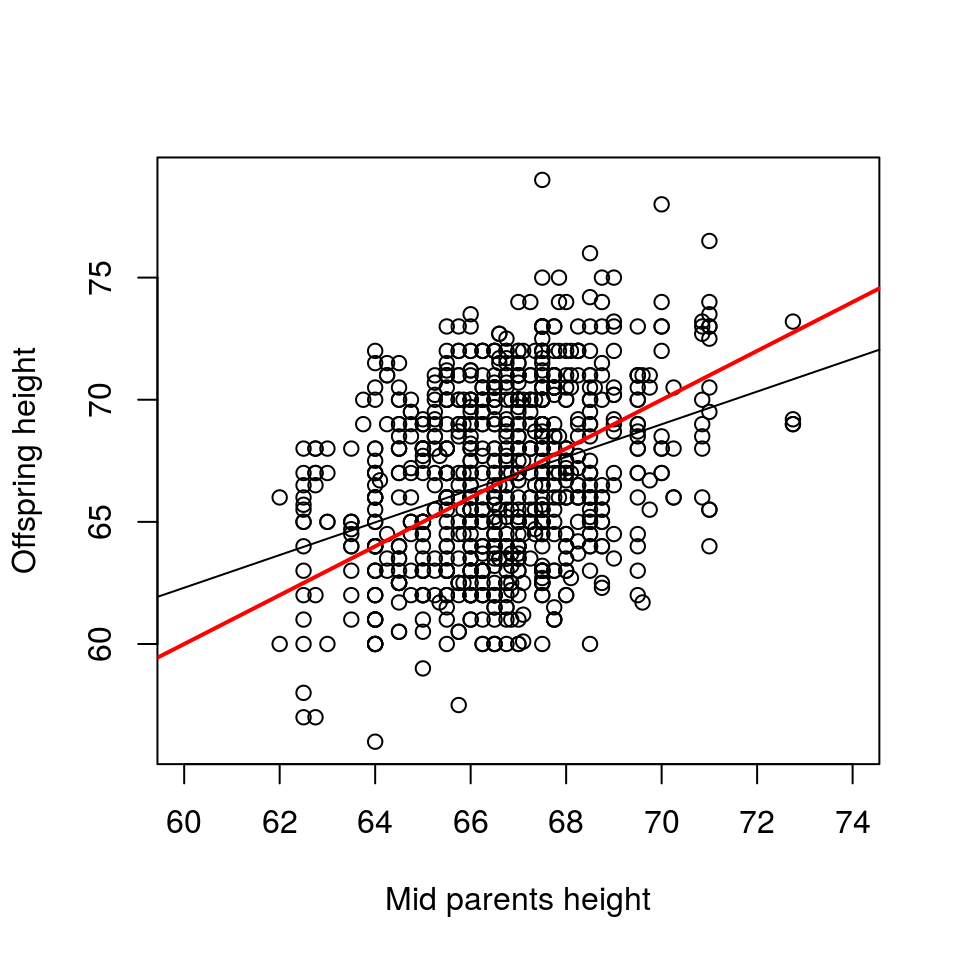
\includegraphics{error-intro-book_files/figure-latex/galton1-1} 

}

\caption{Data drawn from `http://www.math.uah.edu/stat/data/Galton.txt`}\label{fig:galton1}
\end{figure}

\begin{figure}

{\centering 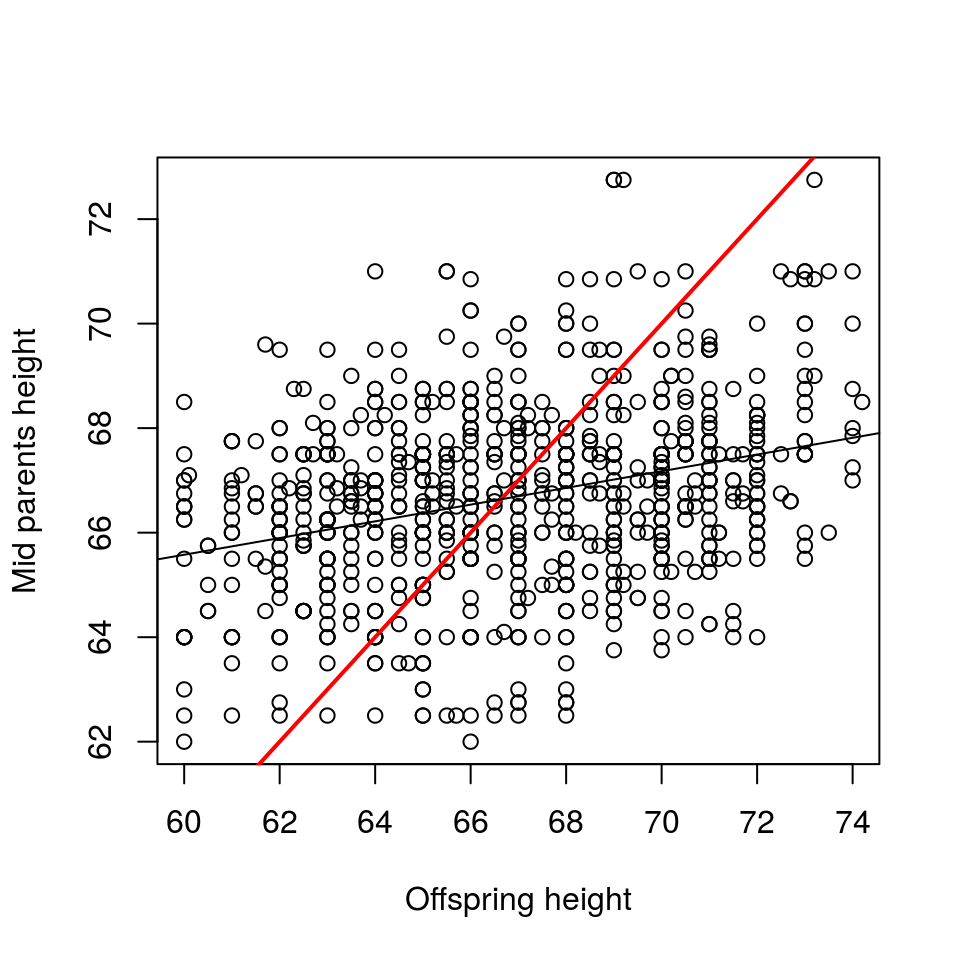
\includegraphics{error-intro-book_files/figure-latex/galton2-1} 

}

\caption{Data drawn from `http://www.math.uah.edu/stat/data/Galton.txt`}\label{fig:galton2}
\end{figure}

The environmental component can be interpreted as the `'measurement
error'', because it is the component that obscures the genetic merit.

\citep{fuller1987, galton1886}

\section{Berkson Measurement Error}\label{berkson-measurement-error}

\section{Error in Categorical and Count
Variables}\label{error-in-categorical-and-count-variables}

\section{Error in the response}\label{error-in-the-response}

\hypertarget{accounting}{\chapter{Methods to Account for Measurement
Error}\label{accounting}}

\section{Bayesian Methods}\label{bayesian-methods}

\section{Simulation Extrapolation
(SIMEX)}\label{simulation-extrapolation-simex}

\chapter{Linear Regression Models}\label{LinReg}

\chapter{Generalized Linear (Mixed) Models}\label{GLMMs}

\section{Classical error}\label{classical-error}

\subsection{Error in a covariate}\label{error-in-a-covariate}

\begin{itemize}
\tightlist
\item
  Correlated covariates
\end{itemize}

\subsection{Error in the response}\label{error-in-the-response-1}

\section{Berkson error}\label{berkson-error}

\subsection{Error in a covariate}\label{error-in-a-covariate-1}

\subsection{Error in the response}\label{error-in-the-response-2}

\chapter{Survival Models}\label{Survival}

\chapter{Advanced Topics}\label{advancedTopics}

\section{Rounding Error}\label{rounding-error}

\section{Misalignement Error in Spatial
Data}\label{misalignement-error-in-spatial-data}

\bibliography{book.bib,packages.bib,literature.bib}


\end{document}
